\chapter{Interacción con el usuario}

\section{Contenidos en parte 3}
\begin{itemize}
    \item Respuesta a cambios en la selección dentro de la tabla.
    \item Añade funcionalidad de los botones añadir, editar, y borrar.
    \item Crear un diálogo emergente (popup dialog) a medida para editar un contacto.
    \item Validación de la entrada del usuario.
\end{itemize}

\section{Respuesta a cambios en la selección de la Tabla}
Todavía no hemos usado la parte derecha de la interfaz de nuestra aplicación. 
La intención es usar esta parte para mostrar los detalles de la persona seleccionada por 
el usuario en la tabla. \\
En primer lugar vamos a añadir un nuevo método dentro de \codigo{PersonOverviewController} que nos ayude a 
rellenar las etiquetas con los datos de una sola persona. \\

Crea un método llamado \codigo{showPersonaDetails(Persona persona)}. Este método recorrerá todas las etiquetas y 
establecerá el texto con detalles de la persona usando \codigo{setText(...)}. Si en vez de una instancia de 
\codigo{Person} se pasa null entonces las etiquetas deben ser borradas. \\

\codigo{PersonOverviewController.java} nuevo método \codigo{showPersonaDetails(Persona persona)}
\begin{minted}[
    linenos,
    numbersep=5pt,
    gobble=0,
    frame=lines,
    framesep=2mm,
    breaklines=true,
    ]{java}

    /**
    * Rellena todos los campos de texto para mostrar detalles sobre la persona.
    * Si la persona especificada es nula, se borran todos los campos de texto.
    * @param persona
    */
   private void showPersonaDetails(Persona persona){
       if(persona != null){
           //Rellene las etiquetas con información del objeto persona.
           nombreLabel.setText(persona.getNombre().get());
           apelidoLabel.setText(persona.getApellido().get());
           calleLabel.setText(persona.getCalle().get());
           codigoPostaLabel.setText(persona.getCodigoPostal().get() + "");
           ciudadLabel.setText(persona.getCiudad().get());
           //¡Necesitamos una forma de convertir el cumpleaños en una Cadena!
           onomasticoLabel.setText(...);
           // onomasticoLabel.setText(DateUtil.format(persona.getOnomastico().get()));
       }else {
           //Si la persona es nula, quitar todo el texto
           nombreLabel.setText("");
           apelidoLabel.setText("");
           calleLabel.setText("");
           codigoPostaLabel.setText("");
           ciudadLabel.setText("");
           onomasticoLabel.setText("");
       }
   }
\end{minted}

\section{Convierte la fecha de nacimiento en una cadena}
Te darás cuenta de que no podemos usar el atributo \codigo{onomastico} directamente 
para establecer el valor de una \codigo{Label} porque se requiere un \codigo{String}, y \codigo{onomastico} es de 
tipo \codigo{LocalDate}. Así pues necesitamos convertir \codigo{onomastico} de \codigo{LocalDate} a \codigo{String}.\\

En la práctica vamos a necesitar convertir entre \codigo{LocalDate} y \codigo{String} en varios sitios y en ambos 
sentidos. Una buena práctica es crear una clase auxiliar con métodos estáticos (\codigo{static}) para esta finalidad. 
Llamaremos a esta clase \codigo{DateUtil} y la ubicaremos una paquete separado denominado \codigo{ch.makery.direcciones.util}:\\

\codigo{DateUtil.java}
\begin{minted}[
    linenos,
    numbersep=5pt,
    gobble=0,
    frame=lines,
    framesep=2mm,
    breaklines=true,
    ]{java}

    package ch.makery.direcciones.util;

    import java.time.LocalDate;
    import java.time.format.DateTimeFormatter;
    
    /**
     * Funciones de ayuda para manejar fechas.
     * @author Marco Jakob
     *
     */
    public class DateUtil {
        /**
         * El patrón de fecha que se utiliza para la conversión.
         * Cambialo como quieras.
         */
        private static final String DATE_PATTERN = "dd-MM-yyyy";
        /**
         * Formateado de fecha
         */
        private static final DateTimeFormatter DATE_FORMATTER =
                DateTimeFormatter.ofPattern(DATE_PATTERN);
        /**
         * Devuelve la fecha que se pasó como parametro en una cadena
         * @param date fecha en formato LocalDate
         * @return fecha en un String
         */
        public static String format(LocalDate date){
            if(date == null){
                return null;
            }
            return DATE_FORMATTER.format(date);
        }
        /**
         * Convierte una cadena en formato de fecha a un objeto LocalDate
         * Retorna nulo si la cadena no pudo convertirse
         *
         * @param dateString fecha como un String
         * @return un objeto de tipo fecha, si no se pudo convertir retorna nulo
         */
        public static LocalDate parse(String dateString){
            try {
                return DATE_FORMATTER.parse(dateString, LocalDate::from);
            } catch (Exception e) {
                return null;
            }
        }
        /**
         * Comprueba la cadena si es una fecha valida
         * @param dateString
         * @return verdadero si la cadena es una fecha valida.
         */
        public static boolean validDate(String dateString){
            //Intenta analizar la cadena
            return DateUtil.parse(dateString) != null;
        }
    }

\end{minted}

\subsection{Utilización de la clase DateUtil}
Ahora necesitamos utilizar la nueva clase \codigo{DateUtil} en el método \codigo{showPersonDetails} de 
\codigo{PersonaOverviewController}. Sustituye el TODO que habíamos añadido con la línea siguiente:

\begin{minted}[
    linenos,
    numbersep=5pt,
    gobble=0,
    frame=lines,
    framesep=2mm,
    breaklines=true,
    ]{java}
    onomasticoLabel.setText(DateUtil.format(persona.getOnomastico().get()));
\end{minted}

\section{Detecta cambios de selección en la tabla}
Para enterarse de que el usuario ha seleccionado a un persona en la tabla de contactos, 
necesitamos escuchar los cambios. Esto se consigue mediante la implementación de un interface de JavaFX 
que se llama \codigo{ChangeListener} con un método llamado \codigo{changed(...)}. Este método solo tiene tres 
parámetros: \codigo{observable}, \codigo{oldValue}, y \codigo{newValue}. \\
En Java 8 la forma más elegante de implementar una interfaz con un único método es mediante una \textit{lambda expression}. 
Añadiremos algunas líneas al método \codigo{initialize()} de \codigo{PersonaOverviewController}. 
El código resultante se asemejará al siguiente:\\
\codigo{PersonOverviewController.java}

\begin{minted}[
    linenos,
    numbersep=5pt,
    gobble=0,
    frame=lines,
    framesep=2mm,
    breaklines=true,
    ]{java}
    /**
	 * Inicializa la clase de controlador
	 * Este método se llama automáticamente después de cargar el archivo fxml.
	 */
	@FXML
	private void initialize(){
		//Inicialice la tabla de personas con las dos columnas.
		nombresColumna.setCellValueFactory(cellData -> cellData.getValue().getNombre());
		apellidosColumna.setCellValueFactory(cellData -> cellData.getValue().getApellido());

		//Limpiar detalles de persona
		showPersonaDetails(null);

		//Escuche los cambios de selección y muestre los detalles de la persona cuando cambie.
		personTable.getSelectionModel().selectedItemProperty().addListener(
				(observable, oldValue, newValue) -> showPersonaDetails(newValue));
	}
\end{minted}

Con \codigo{showPersonDetails(null);} borramos los detalles de una persona.\\
Con \codigo{personaTable.getSelectionModel...} obtenemos la \textit{selectedItemProperty} de la tabla de personas, 
y le añadimos un \textit{listener}. Cuando quiera que el usuario seleccione a una persona en la tabla, 
nuestra \textit{lambda expression} será ejecutada: se toma la persona recien seleccionada y se le pasa al 
método \codigo{showPersonDetails(...)}. \\
Intenta \textbf{ejecutar tu aplicación} en este momento. Comprueba que cuando seleccionas a una persona, 
los detalles sobre esta son mostrados en la parte derecha de la ventana. \\
Si algo no funciona, puedes comparar tu clase \codigo{PersonaOverviewController} con 
\textcolor{azul}{\href{https://github.com/mateomtz199/direccionesapp-part4}{PersonOverviewController.java}}.

\section{El botón de borrar (Delete)}
Nuestro interfaz de usuario ya contiene un botón de borrar, pero sin funcionalidad. Podemos seleccionar la 
acción a ejecutar al pulsar un botón desde el \textit{Scene Builder}. Cualquier método de nuestro controlador 
anotado con \codigo{ @FXML} (o declarado como \textit{public}) es accesible desde \textit{Scene Builder}. 
Así pues, empecemos añadiendo el método de borrado al final de nuestra clase \codigo{PersonaOverviewController}:\\
\codigo{PersonaOverviewController.java}

\begin{minted}[
    linenos,
    numbersep=5pt,
    gobble=0,
    frame=lines,
    framesep=2mm,
    breaklines=true,
    ]{java}
    /**
	 * Se llama cuando el usuario hace clic en el botón Eliminar.
	 */
	@FXML
	private void handleDeletePersona(){
		int selectedIndex = personTable.getSelectionModel().getSelectedIndex();
		personTable.getItems().remove(selectedIndex);
	}
\end{minted}

Ahora, abre el archivo \codigo{PersonOverview.fxml} en el \textit{SceneBuilder}. 
Selecciona el botón \textit{Eliminar}, abre el apartado \textit{Code} y pon \codigo{handleDeletePerson} 
en el menú desplegable denominado \textbf{On Action}.
\begin{figure}[H]
    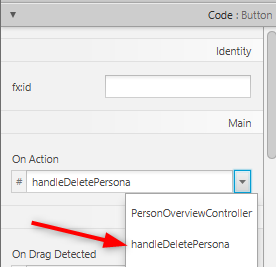
\includegraphics{img/5-handleDeletePerson.png}
\end{figure}

\section{Gestión de errores}
Si ejecutas tu aplicación en este punto deberías ser capaz de borrar personas de la tabla. 
Pero, ¿qué ocurre si pulsas el botón de borrar sin seleccionar a nadie en la tabla.\\
Se produce un error de tipo \codigo{ArrayIndexOutOfBoundsException} porque no puede borrar una persona 
en el índice \codigo{-1}, que es el valor devuelto por el método \codigo{getSelectedIndex()} - 
cuando no hay ningún elemento seleccionado.\\
Ignorar semejante error no es nada recomendable. Deberíamos hacerle saber al usuario que tiene 
que seleccionar una persona previamente para poderla borrar (incluso mejor sería deshabilitar el 
botón para que el usuario ni siquiera tenga la oportunidad de realizar una acción incorrecta).\\

Con algunos cambios en el método \codigo{handleDeletePerson()} podemos mostrar una simple ventana de diálogo 
emergente en el caso de que el usuario pulse el botón Delete sin haber seleccionado a nadie en la 
tabla de contactos:\\
\codigo{PersonOverviewController}
\begin{minted}[
    linenos,
    numbersep=5pt,
    gobble=0,
    frame=lines,
    framesep=2mm,
    breaklines=true,
    ]{java}
    /**
	 * Se llama cuando el usuario hace clic en el botón Eliminar.
	 */
	@FXML
	private void handleDeletePersona(){
		int selectedIndex = personTable.getSelectionModel().getSelectedIndex();
		if(selectedIndex >= 0){
			personTable.getItems().remove(selectedIndex);
		}
		else {
			Alert alert = new Alert(AlertType.WARNING);
			alert.setTitle("Sin seleccion");
			alert.setHeaderText("No has seleccionado una persona");
			alert.setContentText("Por favor selecciona una persona de la lista para eliminar");
			alert.showAndWait();
		}
	}
\end{minted}

\begin{tcolorbox}[leftrule=3mm]
	\textbf{Nota:} Para ver más ejemplos de utilización de ventanas de diálogo, consulta JavaFX 8 Dialogs.
\end{tcolorbox}

\section{Diálogos para crear y editar contactos}
Las acciones de editar y crear nuevo contacto necesitan algo más de elaboración: vamos a 
necesitar una ventana de diálogo a medida (es decir, un nuevo \codigo{stage}) con un formulario 
para preguntar al usuario los detalles sobre la persona.
\subsection{Diseña la ventana de diálogo}
\begin{enumerate}
    \item Crea un nuevo archivo fxml llamado \codigo{PersonEditDialog.fxml} dentro del paquete \textit{view}.
    \item Usa un panel de rejilla (\codigo{GridPane}), etiquetas (\codigo{Label}), campos de texto 
    (\codigo{TextField}) y botones (Button) para crear una ventana de diálogo como la siguiente:
    \begin{figure}[H]
		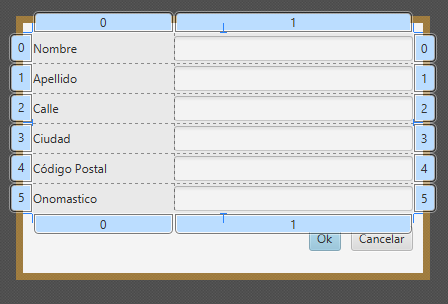
\includegraphics{img/5-VentanaDialogo.png}
	\end{figure}
\end{enumerate}

\subsection{Crear el controlador}
Crea el controlador para la ventana de edición de personas y llámalo \codigo{PersonEditDialogController.java}:\\
\codigo{PersonEditDialogController}
\begin{minted}[
    linenos,
    numbersep=5pt,
    gobble=0,
    frame=lines,
    framesep=2mm,
    breaklines=true,
    ]{java}
    package ch.makery.direcciones.view;

import ch.makery.direcciones.model.Persona;
import ch.makery.direcciones.util.DateUtil;
import javafx.fxml.FXML;
import javafx.scene.control.Alert;
import javafx.scene.control.TextField;
import javafx.scene.control.Alert.AlertType;
import javafx.scene.image.Image;
import javafx.stage.Stage;

/**
 * Diálogo para editar detalles de una persona
 * @author Yo
 *
 */
public class PersonEditDialogController {
	@FXML
	private TextField nombreField;
	@FXML
	private TextField apellidoField;
	@FXML
	private TextField calleField;
	@FXML
	private TextField codigoPostalField;
	@FXML
	private TextField ciudadField;
	@FXML
	private TextField onomasticoField;

	private Stage dialogStage;
	private Persona persona;
	private boolean okClicked = false;
	/**
	 * Inicializa la clase de controlador.
	 * Este método se llama automáticamente después de cargar el archivo fxml.
	 */
	@FXML
	private void initialize(){

	}
	/**
	 * Establece el escenario de este diálogo.
	 * @param dialogStage
	 */
	public void setDialogStage(Stage dialogStage){
		this.dialogStage = dialogStage;
		this.dialogStage.getIcons().add(new Image("file:resources/images/contacto.png"));
	}
	/**
	 * Establece la persona a editar en el diálogo.
	 * @param persona
	 */
	public void setPerson(Persona persona){
		this.persona = persona;
		nombreField.setText(persona.getNombre().get());
		apellidoField.setText(persona.getApellido().get());
		calleField.setText(persona.getCalle().get());
		codigoPostalField.setText(persona.getCodigoPostal().get() + "");
		ciudadField.setText(persona.getCiudad().get());
		onomasticoField.setText(DateUtil.format(persona.getOnomastico().get()));
		onomasticoField.setPromptText("dd-mm-yyyy");
	}
	/**
	 * Devuelve verdadero si el usuario hizo clic en aceptar
	 * falso de lo contrario
	 * @return
	 */
	public boolean isOkClicked(){
		return okClicked;
	}
	/**
	 * Valida la entrada del usuario en los campos de texto.
	 * @return verdadero si la entrada es valida.
	 */
	private boolean isInputValid(){
		String errorMessage = "";

        if (nombreField.getText() == null || nombreField.getText().length() == 0) {
            errorMessage += "El nombre no es valido!\n";
        }
        if (apellidoField.getText() == null || apellidoField.getText().length() == 0) {
            errorMessage += "El apellido no es valido!\n";
        }
        if (calleField.getText() == null || calleField.getText().length() == 0) {
            errorMessage += "La calle no es valido!\n";
        }

        if (codigoPostalField.getText() == null || codigoPostalField.getText().length() == 0) {
            errorMessage += "El código postal no es valido!\n";
        } else {
            // Intenta analizar el código postal en un int
            try {
                Integer.parseInt(codigoPostalField.getText());
            } catch (NumberFormatException e) {
                errorMessage += "El Código Postal no es valido, debe se un entero!\n";
            }
        }

        if (ciudadField.getText() == null || ciudadField.getText().length() == 0) {
            errorMessage += "No valid city!\n";
        }

        if (onomasticoField.getText() == null || onomasticoField.getText().length() == 0) {
            errorMessage += "Onomastico no es valido!\n";
        } else {
            if (!DateUtil.validDate(onomasticoField.getText())) {
                errorMessage += "El onomastico no es valido. Usa el formato dd-mm-yyyy!\n";
            }
        }

        if (errorMessage.length() == 0) {
            return true;
        } else {
            // Mostrar mensaje de error.
        	Alert alert = new Alert(AlertType.WARNING);
			alert.setTitle("Campos no validos");
			alert.setHeaderText("Por favor corrige los campos no validos");
			alert.setContentText(errorMessage);
			alert.showAndWait();
            return false;
        }
	}
	/**
	 * Se llama cuando el usuario hace clic en Aceptar
	 */
	@FXML
	private void handleOk(){
		if(isInputValid()){
			persona.setNombre(nombreField.getText());
			persona.setApellido(apellidoField.getText());
			persona.setCalle(calleField.getText());
			persona.setCodigoPostal(Integer.parseInt(codigoPostalField.getText()));
			persona.setCiudad(ciudadField.getText());
			persona.setOnomastico(DateUtil.parse(onomasticoField.getText()));
			okClicked = true;
			dialogStage.close();
		}
	}
	/**
	 * Se llama cuando el usuario hace clic en cancelar.
	 */
	@FXML
	private void handleCancel(){
		dialogStage.close();
	}
}

	}
\end{minted}

Algunas cuestiones relativas a este controlador:
\begin{itemize}
    \item El método \codigo{setPerson(...)} puede ser invocado desde otra clase para establecer la 
    persona que será editada.
    \item Cuando el usuario pula el botón OK, el método \codigo{handleOk()} es invocado. Primero se valida la 
    entrada del usuario mediante la ejecución del método \codigo{isInputValid()}. Sólo si la validación tiene 
    éxito el objeto persona es modificado con los datos introducidos por el usuario. 
    Esos cambios son aplicados directamente sobre el objeto pasado como argumento del método \codigo{setPerson(...)}!
    \item El método boleano \codigo{okClicked} se utiliza para determinar si el usuario ha pulsado el 
    botón OK o el botón Cancelar.
\end{itemize}

\subsection{Enlaza la vista y el controlador}
Una vez creadas la vista (FXML) y el controlador, necesitamos vincular el uno con el otro:
\begin{enumerate}
    \item Abre el archivo \codigo{PersonEditDialog.fxml}.
    \item En la sección Controller a la izquierda selecciona \codigo{PersonEditDialogController} 
    como clase de control.
    \item Establece el campo \textbf{fx:id} de todas los \codigo{TextField} con los identificadores de los 
    atributos del controlador correspondientes.
    \item Especifica el campo \textbf{onAction} de los dos botones con los métodos del controlador correspondientes a 
    cada acción.
\end{enumerate}
\subsection{Abriendo la ventana de diálogo}
Añade un método para cargar y mostrar el método de edición de una persona dentro de la clase \codigo{MainApp}:
\codigo{MainApp.java}
\begin{minted}[
    linenos,
    numbersep=5pt,
    gobble=0,
    frame=lines,
    framesep=2mm,
    breaklines=true,
    ]{java}
    /**
	 * Abre un cuadro de diálogo para editar detalles para la persona especificada.
	 * Si el usuario hace clic en Aceptar, los cambios se guardan en el objeto
	 * de persona proporcionado y se devuelve verdadero.
	 *
	 * @param persona objeto persona a editar
	 * @return  verdadero si el usuario hizo clic en Aceptar, falso en caso contrario.
	 */
	public boolean showPersonEditDialog(Persona persona){
		try {
			//Cargue el archivo fxml y cree una nueva escena para el
			//cuadro de diálogo emergente.
			FXMLLoader loader = new FXMLLoader();
			loader.setLocation(
					MainApp.class.getResource("view/PersonEditDialog.fxml")
					);
			AnchorPane page = (AnchorPane) loader.load();

			//Crear el cuadro de diálogo de la escena
			Stage dialogStage = new Stage();
			dialogStage.setTitle("Editar persona");
			dialogStage.initModality(Modality.WINDOW_MODAL);
			dialogStage.initOwner(primaryStage);
			Scene scene = new Scene(page);
			dialogStage.setScene(scene);

			//Envia la persona al controlador
			PersonEditDialogController controller = loader.getController();
			controller.setDialogStage(dialogStage);
			controller.setPerson(persona);

			//Muestra el diálogo y espera hasta que el usuario lo cierre.
			dialogStage.showAndWait();

			return controller.isOkClicked();
		} catch (IOException e) {
			e.printStackTrace();
			return false;
		}
	}
\end{minted}
Añade los siguientes métodos a la clase \codigo{PersonOverviewController}. Esos métodos llamarán al método 
\codigo{showPersonEditDialog(...)} desde \codigo{MainApp} cuando el usuario pulse en los botones Nuevo o Editar.\\
\codigo{PersonOverviewController.java}
\begin{minted}[
    linenos,
    numbersep=5pt,
    gobble=0,
    frame=lines,
    framesep=2mm,
    breaklines=true,
    ]{java}
    /**
	 * Se llama cuando el usuario hace clic en el botón Nuevo.
	 * Abre un cuadro de diálogo para editar detalles para una nueva persona.
	 */
	@FXML
	private void handleNewPerson(){
		Persona temPersona = new Persona();
		boolean okClicked = mainApp.showPersonEditDialog(temPersona);
		if(okClicked){
			mainApp.getPersonData().add(temPersona);
		}
	}
	/*
	 * Se llama cuando el usuario hace clic en el botón editar.
	 * Abre un cuadro de diálogo para editar detalles para la persona seleccionada.
	 */
	@FXML
	private void handleEditPerson(){
		Persona personaSeleccionada = personTable.getSelectionModel().getSelectedItem();
		if(personaSeleccionada != null){
			boolean okClicked = mainApp.showPersonEditDialog(personaSeleccionada);
			if(okClicked){
				showPersonaDetails(personaSeleccionada);
			}
		}else {
			Alert alert = new Alert(AlertType.WARNING);
			alert.setTitle("Sin seleccion");
			alert.setHeaderText("No has seleccionado una persona");
			alert.setContentText("Por favor selecciona una persona de la lista para eliminar");
			alert.showAndWait();
		}
	}
\end{minted}
Abre el archivo \codigo{PersonOverview.fxml} mediante \textit{Scene Builder}. 
Elige los métodos correspondientes en el campo \textbf{On Action} para los botones Nuevo y Editar.

\section{¡Ya está!}
Llegados a este punto deberías tener una aplicación de \textit{libreta de contactos} en funcionamiento. 
Esta aplicación es capaz de añadir, editar y borrar personas. Tiene incluso algunas capacidades de 
validación para evitar que el usuario introduzca información incorrecta.\\
Espero que los conceptos y estructura de esta aplicación te permitan empezar tu propia aplicación JavaFX. ¡Disfruta !